%!TEX root = ../Report.tex
\chapter{Hardware}
\section{流水线CPU的实现}
\kaishu
\hspace*{5mm}五级流水线CPU的基本思想即为,将CPU的工作分为:\coloremph{取指-译码-执行-访存-写回}一共
5个阶段,在我们的实验中,我们对于CPU的实现的流程图如下所示:
\begin{figure}[htbp]
    \centering
    \caption{五级流水线CPU流程图}
    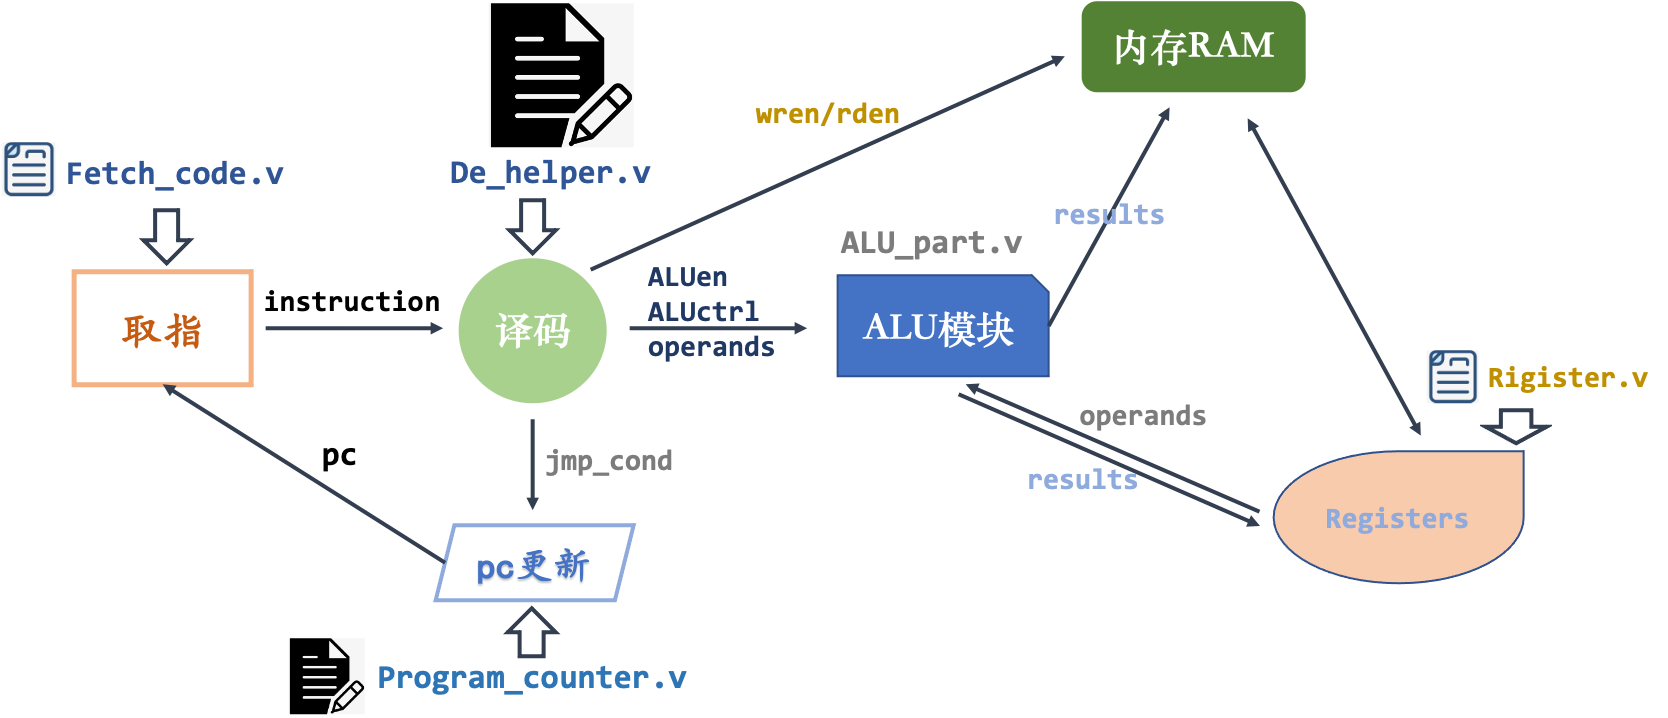
\includegraphics[scale = 0.5]{flowchart.png}
\end{figure}
\songti
下面就分阶段地对于CPU的实现进行介绍。

\rule[-10pt]{14.3cm}{0.05em}
\subsection{取指令}
\hspace*{5mm}取指令阶段是在\file{Fetch\_code.v}中实现。这一阶段是整个CPU\coloremph{工作的基础},只有在指令被
正确取出的前提下,才能取考虑之后的操作是否正确。为了减轻CPU中数据\code{RAM}的工作负担,
也避免时序上与预期产生偏差,我们将代码段(MIPS汇编生成的机器码)存储在一个单独的\code{ROM}——\code{instrtable}中。

\kaishu
\code{Fetch\_code}模块中,输入为时钟信号\code{clk}和一个相对的pc值\code{instr\_addr},输出为
在这个时钟周期需要执行的32位指令的机器码。之所以称作是相对的pc值,是因为在\file{Mars}
汇编器中,指令的编号默认从0x400000开始,而\code{instrtable}中的指令却默认从0开始,所以传进来的
pc与真实的pc相差一个固定的值。

\code{instrtable}使用生成的指令机器码\file{overall.txt}进行初始化。在实际的执行中,一个指令占据4个字节,
所以pc指针一定是4的倍数,而在本模块的\code{ROM}中,因为一个寄存器即为32位,所以指令的真正地址是$\dfrac{pc}{4}$.
故使用\code{instr\_addr[11:2]}进行寻址,得到对应的指令代码传出即可。

代码如下所示:
\begin{lstlisting}[style = verilog-style, caption={module Fetch\_code}]
module Fetch_code(
    input clk,
    output [31:0] instr,
    input [13:0] instr_addr
);
reg [31:0] instrtable [1023:0];
initial 
begin
    $readmemh("overall.txt", instrtable);
end
wire [9:0] pc_in_rom;

assign pc_in_rom = instr_addr[11:2];
assign instr = instrtable[pc_in_rom]; 
// 一个指令4个字节,除以4以后取指令,地址为10位数
endmodule

\end{lstlisting}
\subsection{指令译码}
\songti
\hspace*{5mm}取完指令后,得到一个指令的机器码\code{instr},下面就需要对指令进行译码。在我们的实验中,
本身使用到的指令较少,所以译码阶段也做了简化。在对CPU进行测试的过程中,我们发现按照之前的实现方式,实际执行的结果
与预期结果有差距,所以对译码阶段进行修改,因此出现了和手册中不相符的一些译码。这样做只有在简单的实验,只包含简单
指令的程序之中才能正确工作,若涉及大型程序及实验,需要更加系统的设计。

译码的功能主要在\file{De\_Helper.v}中实现。本模块的主要输入输出引脚如下所示:
\begin{lstlisting}[style = verilog-style, caption={input/output of decode}]
module De_Helper( // only the decode part, no valid signal here
	input [31:0] instr,
	output reg [3:0] jmp_cond,
	output reg RorI, // 0:R type; 1:I type(use immediate). If not used, I as a default type
	output [4:0] rs,
	output [4:0] rt,
	output [4:0] rd,
	output [15:0] imm,
	output [4:0] shamt,
	output reg [3:0] ALUctrl,
	output reg ALUen,
	output reg Memtoreg, //1:load from mem
	output reg Memwr, //1:load to mem
	output [25:0] pcimm
);
\end{lstlisting}

\kaishu
在输入的引脚中,\code{instr}较为显然,是从上一阶段得到的需要译码的指令机器码。译码阶段不需要时钟信号,只要传进来的机器码
有所变化,就会再一次执行所有操作。

输出\code{jmp\_cond}表示跳转状况,这一输出主要为了\file{program\_counter}模块服务,
我们对不同的跳转方式进行编码,这些编码在宏模块\file{ALU.v}中给出:
\begin{lstlisting}[style = verilog-style, caption={Type of jmp\_cond}]
`define NOP 4'b0000
`define BLEZ 4'b0001
`define BEQ  4'b0010
`define BNE 4'b0011
`define J   4'b0100
`define JAL 4'b0101
`define JR 4'b0110
\end{lstlisting}

其中\code{NOP}表示不需要跳转,在这种情况下pc直接加上4即可。剩下的几种条件和相应的指令对应起来,代表着几种不同的跳转情况,
这在\file{program\_counter.v}中有具体的实现。

第二个输出参数\code{RorI}就像注释里说的那样,表示这一条指令是否为I type,如果是的画该输出为1,否则输出为0。

输出引脚\code{rs}, \code{rt}, \code{rd}分别表示两个操作数寄存器的编号和目的寄存器的编号,这个直接从指令中取出即可;
\code{op}表示操作码,\code{func}表示\file{ALU}操作的类型,\code{imm}表示I type指令的操作数,而
\code{pcimm}表示pc直接跳转时所需要的参考地址,这一输出将在\file{program\_counter.v}中使用。\code{shamt}
与手册中的定义一致,用于移位操作。以上这些参数只需要直接从传入的机器码中取出即可。

如下所示:
\begin{lstlisting}[style = verilog-style, caption={Basic decoding}]
assign op  = instr[31:26];
assign func = instr[5:0];
assign rs  = instr[25:21];
assign rt  = instr[20:16];
assign rd  = (op == 6'h3) ? 31 : instr[15:11];
assign imm = instr[15:0];
assign pcimm = instr[25:0];
assign shamt = instr[10:6];
\end{lstlisting}

\lstinline$ALUen$和\lstinline$ALUctrl$主要用于\file{ALU\_part.v}模块的运算,它代表是否需要\lstinline$ALU$计算
以及具体的计算类型。

\lstinline$Memtoreg$和\lstinline$Memwr$分别代表是否是从内存写入寄存器,以及是否需要写入内存。
\\*[1cm]
\songti
下面以几个具体的指令译码为例子,解释一下本模块的具体实现。
当\code{op}为0时,大部分为\file{ALU}操作:
\begin{lstlisting}[style=verilog-style, caption={R type ALU}]
case(op)
6'd0:
///////////////R-type///////////////////////
begin
	if(func == 6'h08)///jr 寄存器
	begin
		RorI<=1'b0;
		ALUen <= 1'b0;
		Memtoreg <= 1'b0;
		Memwr <= 1'b0;
		jmp_cond <= `JR;
	end
	else
	begin
		RorI <= 1'b0;
		ALUen <= 1'b1;
		Memtoreg <= 1'b0;
		Memwr <= 1'b0;
		jmp_cond<=`NOP;
////////Judge the func////////
		case(func)
		6'h20: ALUctrl <= `ADD_op;
		6'h21: ALUctrl <= `ADDU_op;
		6'h22: ALUctrl <= `SUB_op;
		6'h23: ALUctrl <= `SUBU_op;
		6'h27: ALUctrl <= `NOR_op;
		6'h2a: ALUctrl <= `SLT_op;
		6'h2b: ALUctrl <= `SLTU_op;
		6'h00: ALUctrl <= `SLL_op;
		6'h03: ALUctrl <= `SAR_op;
		endcase
	end
end
\end{lstlisting}

\kaishu
在\code{op}为0的时候,需要对\code{func}进行判断来译码。

当\lstinline$func$为0时,这个时候为\code{jr}指令,那么自然:\lstinline{ALUen}为0,同时是
R type,不需要写入寄存器,也不需要读取/写入内存。这时将\lstinline$jmp_cond$设置为\code{`JR}。

除此之外,在其它的\lstinline$func$条件下,均为寄存器类型的\lstinline$ALU$操作,所以首先设置
\code{ALUen <= 1};同时因为是寄存器类型,所以\code{RorI}为0,也不需要操作内存。
ALU操作主要执行运算,所以也不需要跳转,跳转条件为\code{`NOP};

接下来只需要根据对应的\lstinline$func$对计算的类型进行赋值即可。\lstinline$ALU$的不同类型
同样在文件\file{ALU.v}中给出。
\\*[1cm]
\songti
当然,ALU类型的指令除了寄存器类型以外,还有立即数类型,以下是一个I type的ALU运算的指令译码例子:
\begin{lstlisting}[style=verilog-style, caption={I type ALU}]
6'h8: begin
    RorI <= 1'b1;
    ALUen <= 1'b1;
    Memtoreg <= 1'b0;
    Memwr <= 1'b0;
    ALUctrl <= `ADD_op;
    jmp_cond<=`NOP;
end
\end{lstlisting}

\kaishu
在这种情况下,与上一种不同的仅仅在于,\lstinline$RorI$被赋值为高电平,目的是当进行计算时,
选取立即数作为第二操作数而不是寄存器\code{rt}。
\\*[1cm]
\songti
以上主要为\code{ALU}类型的指令,下面介绍访存类型的指令译码。

\kaishu
在涉及内存的指令译码中,最关键的即为两个引脚\code{Memtoreg}和\code{Memwr}:
\begin{lstlisting}[style=verilog-style, caption={Mem type decoding}]
6'h23: begin
    RorI <= 1'b1;// rt 作地址
    Memtoreg <= 1'b1;
    Memwr <= 1'b0;
    ALUen <= 1'b0;
    jmp_cond<=`NOP;
end
6'h2b: begin
    RorI <= 1'b1;
    Memtoreg <= 1'b0;
    Memwr <= 1'b1;
    ALUen <= 1'b0;
    jmp_cond<=`NOP;
end
\end{lstlisting}

很容易知道,以上两个指令分别为\code{lw}和\code{sw},分别表示从寄存器写入内存,和从内存写入寄存器。
\\*[0.5cm]
\songti
对于跳转类型的指令,最重要的是给跳转条件赋予正确的类型,同时,对于该跳转地址计算所需要的参数,也需要译码得出。
\kaishu
例如直接跳转类型:
\begin{lstlisting}[style=verilog-style, caption={Jump type decoding}]
6'h2: begin  //j
    RorI <= 1'b0;
    ALUen <= 1'b0;
    Memtoreg <= 1'b0;
    Memwr <= 1'b0;
    jmp_cond <= `J;
end
\end{lstlisting}
\subsection{指令执行}
\songti
正如前面所分析的那样,我们并没有写一个专门的执行模块,因为对于不同类型的指令,它的执行操作不一样,执行方式也不一样。
\\*[0.5cm]
指令类型有计算,跳转和访存等,所以我们在\file{ALU\_part.v}模块进行计算,在\file{program\_counter.v}模块中进行pc跳转。
\\*[0.5cm]
对于计算模块,即\file{ALU\_part.v},并没有什么需要解释的,只需要按照译码的类型进行相应的计算即可。
\\*[0.5cm]
下面来介绍一下pc模块。
\begin{lstlisting}[style=verilog-style, caption={program counter}]
wire [31:0] seq_pc,signed_offset;
initial begin
    pc_state = 32'h400000;
end
assign signed_offset = {{14{J_branch_offset[15]}},J_branch_offset,2'b0};
assign seq_pc = pc_state + 4;
always @ (posedge pc_clk)
begin
    if (reset) pc_state <= 32'h400000;
    else begin case (jmp_type)
        ......//根据不同的跳转类型给pc赋予对应的值,此处不再赘述。
        default : pc_state <= seq_pc;
        endcase
    end
end
\end{lstlisting}

\kaishu
\file{program.v}模块主要负责指令结束后pc的跳转位置。根据代码可以看出,我们对于pc的控制取决于传入的\code{jmp\_cond}和\code{cmp\_res},
对于每一种跳转条件均给予考虑。在分支跳转的情况中,我们需要考虑比较结果,如果满足,则pc的位置跳转到
\code{seq\_pc}加上带符号偏移量的位置,否则顺序执行。对于直接跳转,则直接跳转到指定的位置。对于不需要跳转的情况,则pc变化为\code{seq\_pc}。


需要注意的一点是,对于给出的关于pc跳转的立即数,在分支跳转中是有符号数,且所有的立即数都需要左移两位。
\subsection{内存与数据RAM}
\songti
我们使用RAM来实现内存的功能,并通过它来实现访存功能。下表展示了在内存中数据段的划分方式。
\\*[0.2cm]
\begin{table}
	\centering
	\caption{数据段的划分}
	\renewcommand\arraystretch{1.5}
	\kaishu
	\begin{tabular}{ccc}  
		\toprule[1pt]  
		\rowcolor[gray]{0.9}   地址空间 &存储内容&详细\\  
		\midrule  
		0x0-0x500&键盘数据存储空间&键盘\texttt{RAM, A port}输入\\
		0x500-0x1000&欢迎界面的信息&事先存储,\texttt{.mif}初始化\\
		0x1000-0x1500&一些帮助信息&\texttt{.mif}初始化\\
		0x1500-0x1700&一些指令的输出信息&事先存储\\
		0x1700-0x2000&指令名称&用于\code{\_strcmp}阶段进行比较\\
		0x2000-0x3000&软件计算信息&\texttt{CPU}计算过程中使用\\
		0x3000- &堆栈空间&\texttt{CPU}运行过程中的栈空间\\ 
		\bottomrule[1pt]  
		\end{tabular} 
\end{table}

\kaishu
对于数据\lstinline$RAM$,我们使用真双口\lstinline$RAM$,\texttt{A port}留给键盘与\texttt{CPU}进行交互,
一部分留给\texttt{CPU}对于内存进行读写。

\subsection{寄存器模块}
\songti
\hspace*{7mm}在寄存器模块中,完成了最后的写回阶段。\file{Registers.v}中使用32个寄存器实现,主要代码如下:
\begin{lstlisting}[style = verilog-style, caption = {Register.v主要实现}]
reg [31:0] regs_all [31:0];
integer i;
initial
begin
    for (i = 0; i <= 31; i = i + 1)
    begin
        regs_all[i] = 0;
    end
end
always @ (posedge clk)
begin
    if (wr_en) regs_all[wr_addr] <= wr_data;
end
\end{lstlisting}

\section{指令实现}
\songti
\hspace*{5mm}本实验中,我们主要实现了如下所示的指令:

\begin{table}
	\centering
	\caption{实现的指令}
	\renewcommand\arraystretch{1.5}
	\kaishu
	\begin{tabular}{cc}  
		\toprule[1pt]  
		\rowcolor[gray]{0.9}   指令类型 & 指令罗列\\  
		\midrule  
		运用ALU计算&\texttt{add addi sub subi and andi or ori xor xori slt sll sra}\\
		访存&\texttt{lw sw}\\
		分支/跳转&\texttt{beq bne ble blez jal j jr}\\
		\bottomrule[1pt]  
		\end{tabular} 
\end{table}

\kaishu
以上指令的执行过程主要是按照上一模块中介绍的五个阶段取执行,在\file{CPU\_overall.v}中,我们对于以上的五个阶段进行了整合,
下面是对于一些关键引脚的赋值:
\begin{lstlisting}[style = verilog-style, caption = {CPU主模块对于一些引脚的分配}]
assign rtnum = RorI ? imm : rd_data2;
assign rsnum = rd_data1;
assign wr_data = ALUen ? rdnum : 
		jmp_cond == `JAL ? pc + 4 : 
		Memtoreg ?mem_fetch : // mem_fetch是从内存中取出的
		0;
assign wr_en = (ALUen | jmp_cond == `JAL | Memtoreg); // 是否需要写入寄存器
assign mem_addr = rd_data1 + imm; // 但是实际上,imm用的都是0
assign mem_save = rd_data2; // 写入内存;
assign wrmem_en = (Memwr) & (~Memtoreg); // CPU是否需要写入内存,用于B port
assign rdmem_en = ~ wrmem_en;
assign wr_addr = (Memtoreg|RorI) ? rt : rd;
assign cmp_res = (rsnum == rtnum) ? 0 : (rsnum < rtnum) ? 1 : 2;
\end{lstlisting}

这些引脚会传入各个模块。

其中\code{wr\_en}和\code{wr\_data}对应的是寄存器模块,表示是否有寄存器需要写入,以及具体写入的值为多少。

而\code{mem\_addr}和\code{mem\_save}, \code{wrmem\_en}则对应的是内存,表示内存是否需要写入,写入的地址
,写入的值具体是多少,都会通过\texttt{CPU}计算出。

\code{rt\_num}和\code{rs\_num}分别表示传给\texttt{ALU}进行计算的操作数1和操作数2。在立即数类型下
,操作数2为立即数。
\subsection{计算指令}

\songti
\hspace*{9mm}计算指令主要有以下所列出的这些,他们主要通过\file{ALU\_part.v}来实现。

在译码阶段,给出\texttt{ALU\_en}和\texttt{ALU\_ctrl}传入到主模块,这决定了是否使用
\texttt{ALU}以及进行何种运算。在主模块中,根据译码阶段给出的信息。再从寄存器模块取出对应的操作数。
计算结束后再次根据\code{wr\_en}决定是否写会寄存器。
\begin{lstlisting}[style = verilog-style, caption = {寄存器读取数据}]
assign rd_data1 = regs_all[rd_addr1];
assign rd_data2 = regs_all[rd_addr2];
\end{lstlisting}


\begin{table}
	\centering
	\caption{计算指令}
	\renewcommand\arraystretch{1.5}
	\kaishu
	\begin{tabular}{cccc}  
		\toprule[1pt]  
		\rowcolor[gray]{0.9}   指令名称 & 操作 &指令名称 &操作\\  
		\midrule  
		\texttt{add} & rd$\gets$ rs + rt &\texttt{addi} & rd$\gets$ rs + imm \\
		\texttt{sub} & rd$\gets$ rs - rt &\texttt{subi} & rd$\gets$ rs - imm \\
		\texttt{and} & rd$\gets$ rs \& rt &\texttt{andi} & rd$\gets$ rs \& imm \\
		\texttt{or} & rd$\gets$ rs | rt &\texttt{ori} & rd$\gets$ rs | imm \\
		\texttt{xor} & rd$\gets$ rs $\oplus$ rt &\texttt{xori} & rd$\gets$ rs $\oplus$ imm \\
		\texttt{sll} & rd$\gets$ rs << shamt &\texttt{sra} & rd$\gets$ rs >> shamt\\
		\texttt{slt} & rd$\gets$ \$\texttt{signed(rs)} < \$\texttt{signed(rt)} &&\\
		\bottomrule[1pt]  
		\end{tabular} 
\end{table}
\subsection{访存指令}
\songti
\hspace*{9mm}访存指令有以下两种:
\begin{table}[htbp]
	\centering
	\caption{访存指令}
	\renewcommand\arraystretch{1.5}
	\kaishu
	\begin{tabular}{cc}  
		\toprule[1pt]  
		\rowcolor[gray]{0.9}   指令名称 & 操作\\  
		\midrule  
		\texttt{sw \$n, imm(\$m)} & 将\$n中的值存储到\$m + imm的位置\\
		\texttt{lw \$n, imm(\$m)} & 将\$m + imm的位置内存中的值加载到\$n寄存器中\\
		\bottomrule[1pt]  
		\end{tabular} 
\end{table}

\songti
通过以下的内存模块实现:
\begin{lstlisting}[style = verilog-style, caption = {数据RAM的访问存储}]
data_ram rd_wr_data(
	.address_a(key_wr_addr), .clock_a(wr_clk), .data_a(wr_ram_data),
	.wren_a(key_wr_en), 
	.address_b(mem_addr), .clock_b(clk50), .data_b(mem_save),
	.wren_b(wrmem_en), .q_b(mem_fetch)
); // 添加一个真双口RAM,一个给键盘一个给CPU
\end{lstlisting}
\subsection{跳转指令}
\hspace*{9mm}跳转指令主要通过上文交代的\file{program\_counter.v}模块计算得出。

主要实现的跳转指令如下所示:

\begin{table}[htbp]
	\centering
	\caption{跳转指令指令}
	\renewcommand\arraystretch{1.5}
	\kaishu
	\begin{tabular}{cc}  
		\toprule[1pt]  
		\rowcolor[gray]{0.9}   指令名称 & 操作\\  
		\midrule  
		\texttt{j imm} & \texttt{pc $\gets$ \{seq\_pc[31:28],imm, 2'b0\}};\\
		\texttt{jr \$n} & \texttt{pc $\gets$ \$n};\\
		\texttt{jal imm} & \texttt{pc $\gets$ \{seq\_pc[31:28],imm, 2'b0\}};\\
		\texttt{beq rs, rt, offset} & \texttt{pc $\gets$ seq\_pc + signed\_offset} if rs = rt\\
		\texttt{bne rs, rt, offset} & \texttt{pc $\gets$ seq\_pc + signed\_offset} if rs $\neq$ rt\\
		\texttt{ble rs, rt, offset} & \texttt{pc $\gets$ seq\_pc + signed\_offset} if rs $\leq$ rt\\
		\bottomrule[1pt]  
		\end{tabular} 
\end{table}

\songti
实际的MIPS指令集中并没有\code{ble}指令,但是在\file{Mars}汇编器中是允许存在的,它将被编译成以下两条指令:

\begin{center}
\coloremph{\texttt{slt \$1, \$2, \$3}}\\
\coloremph{\texttt{beq \$1, \$0, imm}}
\end{center}

所以我们在汇编中使用了\code{ble}这条指令,它可以使得一些跳转条件更方便表示。

\kaishu
对于\code{jr}指令,我们将从寄存器模块中取出对应的跳转寄存器,然后传入pc模块,根据跳转条件判断是否要跳到该寄存器存储的位置。

对于\code{jal}指令,我们不仅要执行与\code{j}指令相同的操作,还需要将返回地址存入\code{\$ra}寄存器,
这个时候我们要求在主模块将\texttt{wr\_addr}赋值为31,并要求寄存器写入使能即可。

对于分支跳转指令,我们将会通过\texttt{ALU}计算出是否需要跳转,并将结果传入pc模块。

\section{IO}
\songti
\hspace*{9mm}本模块介绍实验中使用的输入输出模块是如何与\texttt{CPU}进行交互的。

为了简化实验,我们并没有实现系统的MMIO,而是选择通过寄存器与输入输出设备进行交互,如何交互将会在软件阶段给予介绍。
这里给出寄存器模块中的一些引脚赋值:
\begin{lstlisting}[style = verilog-style, caption = {寄存器与IO交互}]
assign vga_addr = (regs_all[21] << 6) + (regs_all[21] << 2) + (regs_all[21] << 1) + regs_all[22];
assign vga_ascii = regs_all[4][10:0];
assign vga_refresh = (regs_all[23] != 0 && regs_all[4][7:0] != 8'h0d);
assign cursor_en = (regs_all[6] != 0);
assign row = regs_all[16][9:0];
assign ram_wr_addr = regs_all[28]; //gp: 写入字符串的位置
assign piano_en = (regs_all[24] == 2);
\end{lstlisting}

从这里导出的\code{ram\_wr\_addr}表示键盘的写入地址,它将会传入数据\texttt{RAM}的A端口,
用于键盘传入的字符的写入。

从这里导出的\code{piano\_en}表示音频模块的使能,它将会直接传入音频模块进行控制。

从这里导出的其它引脚,均用来控制\texttt{VGA}:
\begin{itemize}
	\item \code{vga\_addr}表示写入显存的地址,用来在屏幕上输出字符;
	\item \code{vga\_ascii}表示写到屏幕上的字符;
	\item \code{vga\_refresh}表示是否需要写入到屏幕上;
	\item \code{cursor\_en}表示当前是否需要显示光标,因为在我们的实验中,开机界面是不需要显示光标的;
	\item \code{row}表示屏幕上移了多少行。
\end{itemize}

在VGA中,也利用这些引脚来实现一定的功能:

\coloremph{\texttt{assign new\_ascii = (vga\_addr != wr\_addr) ? ascii : (cursor \&\& cursor\_en) ? 8'h5f : 8'h0;}}


这里将利用光标使能和光标时钟来显示光标。
\\*[0.2cm]
\kaishu
我们还在屏幕上输出了不同的颜色的字符。具体的实现方案是,对于8位字符码,我们扩展到11位,高三位表示
该要显示的颜色序号,具体的颜色我们根据序号存储在VGA模块的寄存器中:
\begin{lstlisting}[style = verilog-style, caption = {字符颜色列表}]
color_list[7] = 24'h6d6875;
color_list[6] = 24'h2a9d8f;
color_list[5] = 24'h264653;
color_list[4] = 24'h7ea7;
color_list[3] = 24'hbb4c30;
color_list[2] = 24'hc47335;
color_list[1] = 24'hff;
color_list[0] = 24'h264653;
\end{lstlisting}

如下所示更改字符颜色:
\begin{lstlisting}[style = verilog-style, caption = {控制字符颜色}]
assign vga_color = color_list[new_ascii[10:8]];
wire font_valid = (font_data[dx] == 1) ? 1 : 0;
assign vr = font_valid ? vga_color[23:16] : bg_r;
assign vg = font_valid ? vga_color[15:8] : bg_g;
assign vb = font_valid ? vga_color[7:0] : bg_b;
\end{lstlisting}
\section{\textsc{CPU TESTS}}
\songti
\hspace*{9mm}在一开始的运行过程中,我们遇到了各种各样的问题,于是编写了较多的测试文件,对项目的各个模块进行测试。

测试使用汇编在目录\file{CPU\_overall$\setminus$instructions}目录下,列表如下:

\begin{table}[htbp]
	\centering
	\caption{测试文件}
	\renewcommand\arraystretch{1.5}
	\kaishu
	\begin{tabular}{cc}  
		\toprule[1pt]  
		\rowcolor[gray]{0.9}   硬件 & 软件\\  
		\midrule  
		\texttt{hex.asm} & \texttt{welcome.asm};\\
		\texttt{read\_key.asm} & \texttt{audio\_new.asm}\\
		\texttt{key\_vga.asm} & \texttt{fibbonacci.asm}\\
		\texttt{vga\_test.asm} & \texttt{fib\_key\_vga.asm}\\
		\texttt{audio\_test.asm} & \texttt{print\_res.asm}\\
		\bottomrule[1pt]  
		\end{tabular} 
\end{table}
\section{遇到的问题和解决方法}
\subsection{与IO之间的交互}

\songti
起初我们的输入输出设备并不能正常工作。而在最开始我们并不知道是哪个地方除了问题:硬件,IO还是汇编代码。

解决方法:\kaishu 我们主要采取\coloremph{逐步排查}的方法,在涉及对\texttt{CPU}进行排查的过程,将\texttt{CPU}的时钟改为\code{KEY[0]},
方便我们观察系统的变化。
\begin{itemize}
	\item 脱离\texttt{CPU}对输入输出设备进行单独调试,若没有问题,进入下一步骤;
	\item 编写更简单的汇编代码,即测试代码,脱离其它软件以及过程的干扰,若不存在问题进入下一步骤;
	\item 将\texttt{CPU}的时钟调整为\code{KEY[0]},将指令的地址、操作数,计算结果导出到七段数码管上。因为数码管数量有限,所以优先选择关键引脚导出,再利用\code{LED}等,\coloremph{高效利用资源调试}。
\end{itemize}
\subsection{VGA显示不够清晰}
\songti
在最开始,我们的屏幕上不能显示稳定的、没有阴影的字符;在后来的软件测试过程中,经常因为少量汇编代码的变动而使得字符出现阴影。

解决方法:\kaishu 我们在调试过程中采取了这样的策略:
\begin{itemize}
	\item 简化\file{VGA.v}模块中的计算与操作,将对于坐标的计算加入到像素点坐标变化的过程中,而不是根据像素点进行乘除法操作;
	\item 在编写汇编代码的过程中,尽量不要在较短的距离内修改同一个寄存器的值。
\end{itemize}
\subsection{CPU无法正确计算简单的程序}
\songti
最开始时,系统甚至无法完成显示\code{HEX}的功能。

解决方法:\kaishu 将一段小程序执行过程中涉及的指令依次排查,按照\coloremph{取指-译码-执行-访存-写回}的过程依次检查各个模块,
按照手册进行检查。

最终发现,我们对于一些指令的操作数以及目的数的赋值有误。

再进行一系列的测试后,我们将所有的指令进行分配,每人排查一部分,努力确保每一条指令都能正确执行。
\section{得到的启示}
\songti
\coloremph{\textbf{机器永远是对的。}}
\\*[0.2cm]
\kaishu
在进行这个实验的过程中,我们经常会不理解开发板的迷惑操作,较为复杂的时序电路是我们所不能理解的,但最终经过调试,
都是我们不小心而犯下的错误。
\\*[0.3cm]
\songti
\textbf{团队合作项目一定要加强沟通。}
\\*[0.2cm]
\kaishu
在最初的调试过程中,我们发现,许多所谓的\texttt{bug}都是源于没有沟通好各自负责的模块之间的协调,各个模块之间的\texttt{API}
没有对应上。
\\*[0.3cm]
\songti
\textbf{积极的\coloremph{RTFM},\coloremph{STFW}。}
\\*[0.2cm]
\kaishu
在实验过程中,关于指令实现问题,都需要寻找官方的\href{http://www.cs.cornell.edu/courses/cs3410/2008fa/MIPS_Vol1.pdf}{\file{MIPS manual}},按照手册执行,而不是根据字面意思进行猜测。
\\关于\texttt{verilog}和\texttt{Quartus}的问题都可以在网络上寻找到答案。
